\documentclass[1p]{elsarticle_modified}
%\bibliographystyle{elsarticle-num}

%\usepackage[colorlinks]{hyperref}
%\usepackage{abbrmath_seonhwa} %\Abb, \Ascr, \Acal ,\Abf, \Afrak
\usepackage{amsfonts}
\usepackage{amssymb}
\usepackage{amsmath}
\usepackage{amsthm}
\usepackage{scalefnt}
\usepackage{amsbsy}
\usepackage{kotex}
\usepackage{caption}
\usepackage{subfig}
\usepackage{color}
\usepackage{graphicx}
\usepackage{xcolor} %% white, black, red, green, blue, cyan, magenta, yellow
\usepackage{float}
\usepackage{setspace}
\usepackage{hyperref}

\usepackage{tikz}
\usetikzlibrary{arrows}

\usepackage{multirow}
\usepackage{array} % fixed length table
\usepackage{hhline}

%%%%%%%%%%%%%%%%%%%%%
\makeatletter
\renewcommand*\env@matrix[1][\arraystretch]{%
	\edef\arraystretch{#1}%
	\hskip -\arraycolsep
	\let\@ifnextchar\new@ifnextchar
	\array{*\c@MaxMatrixCols c}}
\makeatother %https://tex.stackexchange.com/questions/14071/how-can-i-increase-the-line-spacing-in-a-matrix
%%%%%%%%%%%%%%%

\usepackage[normalem]{ulem}

\newcommand{\msout}[1]{\ifmmode\text{\sout{\ensuremath{#1}}}\else\sout{#1}\fi}
%SOURCE: \msout is \stkout macro in https://tex.stackexchange.com/questions/20609/strikeout-in-math-mode

\newcommand{\cancel}[1]{
	\ifmmode
	{\color{red}\msout{#1}}
	\else
	{\color{red}\sout{#1}}
	\fi
}

\newcommand{\add}[1]{
	{\color{blue}\uwave{#1}}
}

\newcommand{\replace}[2]{
	\ifmmode
	{\color{red}\msout{#1}}{\color{blue}\uwave{#2}}
	\else
	{\color{red}\sout{#1}}{\color{blue}\uwave{#2}}
	\fi
}

\newcommand{\Sol}{\mathcal{S}} %segment
\newcommand{\D}{D} %diagram
\newcommand{\A}{\mathcal{A}} %arc


%%%%%%%%%%%%%%%%%%%%%%%%%%%%%5 test

\def\sl{\operatorname{\textup{SL}}(2,\Cbb)}
\def\psl{\operatorname{\textup{PSL}}(2,\Cbb)}
\def\quan{\mkern 1mu \triangleright \mkern 1mu}

\theoremstyle{definition}
\newtheorem{thm}{Theorem}[section]
\newtheorem{prop}[thm]{Proposition}
\newtheorem{lem}[thm]{Lemma}
\newtheorem{ques}[thm]{Question}
\newtheorem{cor}[thm]{Corollary}
\newtheorem{defn}[thm]{Definition}
\newtheorem{exam}[thm]{Example}
\newtheorem{rmk}[thm]{Remark}
\newtheorem{alg}[thm]{Algorithm}

\newcommand{\I}{\sqrt{-1}}
\begin{document}

%\begin{frontmatter}
%
%\title{Boundary parabolic representations of knots up to 8 crossings}
%
%%% Group authors per affiliation:
%\author{Yunhi Cho} 
%\address{Department of Mathematics, University of Seoul, Seoul, Korea}
%\ead{yhcho@uos.ac.kr}
%
%
%\author{Seonhwa Kim} %\fnref{s_kim}}
%\address{Center for Geometry and Physics, Institute for Basic Science, Pohang, 37673, Korea}
%\ead{ryeona17@ibs.re.kr}
%
%\author{Hyuk Kim}
%\address{Department of Mathematical Sciences, Seoul National University, Seoul 08826, Korea}
%\ead{hyukkim@snu.ac.kr}
%
%\author{Seokbeom Yoon}
%\address{Department of Mathematical Sciences, Seoul National University, Seoul, 08826,  Korea}
%\ead{sbyoon15@snu.ac.kr}
%
%\begin{abstract}
%We find all boundary parabolic representation of knots up to 8 crossings.
%
%\end{abstract}
%\begin{keyword}
%    \MSC[2010] 57M25 
%\end{keyword}
%
%\end{frontmatter}

%\linenumbers
%\tableofcontents
%
\newcommand\colored[1]{\textcolor{white}{\rule[-0.35ex]{0.8em}{1.4ex}}\kern-0.8em\color{red} #1}%
%\newcommand\colored[1]{\textcolor{white}{ #1}\kern-2.17ex	\textcolor{white}{ #1}\kern-1.81ex	\textcolor{white}{ #1}\kern-2.15ex\color{red}#1	}

{\Large $\underline{12a_{0096}~(K12a_{0096})}$}

\setlength{\tabcolsep}{10pt}
\renewcommand{\arraystretch}{1.6}
\vspace{1cm}\begin{tabular}{m{100pt}>{\centering\arraybackslash}m{274pt}}
\multirow{5}{120pt}{
	\centering
	\includegraphics[width=112pt]{../../../GIT/diagram.site/Diagrams/png/897_12a_0096.png}\\
\ \ \ A knot diagram\footnotemark}&
\allowdisplaybreaks
\textbf{Linearized knot diagam} \\
\cline{2-2}
 &
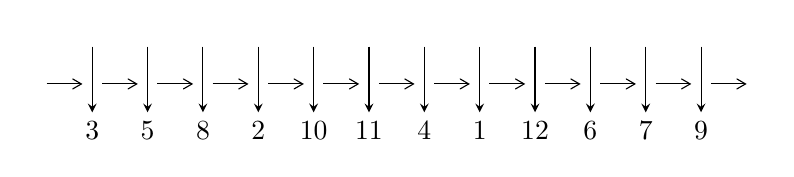
\begin{tikzpicture}[x=20pt, y=17pt]
	% nodes
	\node (C0) at (0, 0) {};
	\node (C1) at (1, 0) {};
	\node (C1U) at (1, +1) {};
	\node (C1D) at (1, -1) {3};

	\node (C2) at (2, 0) {};
	\node (C2U) at (2, +1) {};
	\node (C2D) at (2, -1) {5};

	\node (C3) at (3, 0) {};
	\node (C3U) at (3, +1) {};
	\node (C3D) at (3, -1) {8};

	\node (C4) at (4, 0) {};
	\node (C4U) at (4, +1) {};
	\node (C4D) at (4, -1) {2};

	\node (C5) at (5, 0) {};
	\node (C5U) at (5, +1) {};
	\node (C5D) at (5, -1) {10};

	\node (C6) at (6, 0) {};
	\node (C6U) at (6, +1) {};
	\node (C6D) at (6, -1) {11};

	\node (C7) at (7, 0) {};
	\node (C7U) at (7, +1) {};
	\node (C7D) at (7, -1) {4};

	\node (C8) at (8, 0) {};
	\node (C8U) at (8, +1) {};
	\node (C8D) at (8, -1) {1};

	\node (C9) at (9, 0) {};
	\node (C9U) at (9, +1) {};
	\node (C9D) at (9, -1) {12};

	\node (C10) at (10, 0) {};
	\node (C10U) at (10, +1) {};
	\node (C10D) at (10, -1) {6};

	\node (C11) at (11, 0) {};
	\node (C11U) at (11, +1) {};
	\node (C11D) at (11, -1) {7};

	\node (C12) at (12, 0) {};
	\node (C12U) at (12, +1) {};
	\node (C12D) at (12, -1) {9};
	\node (C13) at (13, 0) {};

	% arrows
	\draw[->,>={angle 60}]
	(C0) edge (C1) (C1) edge (C2) (C2) edge (C3) (C3) edge (C4) (C4) edge (C5) (C5) edge (C6) (C6) edge (C7) (C7) edge (C8) (C8) edge (C9) (C9) edge (C10) (C10) edge (C11) (C11) edge (C12) (C12) edge (C13) ;	\draw[->,>=stealth]
	(C1U) edge (C1D) (C2U) edge (C2D) (C3U) edge (C3D) (C4U) edge (C4D) (C5U) edge (C5D) (C6U) edge (C6D) (C7U) edge (C7D) (C8U) edge (C8D) (C9U) edge (C9D) (C10U) edge (C10D) (C11U) edge (C11D) (C12U) edge (C12D) ;
	\end{tikzpicture} \\
\hhline{~~} \\& 
\textbf{Solving Sequence} \\ \cline{2-2} 
 &
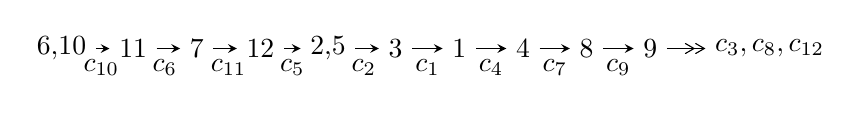
\begin{tikzpicture}[x=23pt, y=7pt]
	% node
	\node (A0) at (-1/8, 0) {6,10};
	\node (A1) at (1, 0) {11};
	\node (A2) at (2, 0) {7};
	\node (A3) at (3, 0) {12};
	\node (A4) at (65/16, 0) {2,5};
	\node (A5) at (41/8, 0) {3};
	\node (A6) at (49/8, 0) {1};
	\node (A7) at (57/8, 0) {4};
	\node (A8) at (65/8, 0) {8};
	\node (A9) at (73/8, 0) {9};
	\node (C1) at (1/2, -1) {$c_{10}$};
	\node (C2) at (3/2, -1) {$c_{6}$};
	\node (C3) at (5/2, -1) {$c_{11}$};
	\node (C4) at (7/2, -1) {$c_{5}$};
	\node (C5) at (37/8, -1) {$c_{2}$};
	\node (C6) at (45/8, -1) {$c_{1}$};
	\node (C7) at (53/8, -1) {$c_{4}$};
	\node (C8) at (61/8, -1) {$c_{7}$};
	\node (C9) at (69/8, -1) {$c_{9}$};
	\node (A10) at (11, 0) {$c_{3},c_{8},c_{12}$};

	% edge
	\draw[->,>=stealth]	
	(A0) edge (A1) (A1) edge (A2) (A2) edge (A3) (A3) edge (A4) (A4) edge (A5) (A5) edge (A6) (A6) edge (A7) (A7) edge (A8) (A8) edge (A9) ;
	\draw[->>,>={angle 60}]	
	(A9) edge (A10);
\end{tikzpicture} \\ 

\end{tabular} \\

\footnotetext{
The image of knot diagram is generated by the software ``\textbf{Draw programme}" developed by Andrew Bartholomew(\url{http://www.layer8.co.uk/maths/draw/index.htm\#Running-draw}), where we modified some parts for our purpose(\url{https://github.com/CATsTAILs/LinksPainter}).
}\phantom \\ \newline 
\centering \textbf{Ideals for irreducible components\footnotemark of $X_{\text{par}}$} 
 
\begin{align*}
I^u_{1}&=\langle 
- u^{59}+31 u^{57}+\cdots-4 u^2+b,\;- u^{62}- u^{61}+\cdots+a-1,\;u^{63}+2 u^{62}+\cdots+2 u-1\rangle \\
I^u_{2}&=\langle 
u^4-2 u^2+b+2 u,\;- u^5+3 u^3+a+1,\;u^6+u^5-3 u^4-2 u^3+2 u^2- u-1\rangle \\
\\
\end{align*}
\raggedright * 2 irreducible components of $\dim_{\mathbb{C}}=0$, with total 69 representations.\\
\footnotetext{All coefficients of polynomials are rational numbers. But the coefficients are sometimes approximated in decimal forms when there is not enough margin.}
\newpage
\renewcommand{\arraystretch}{1}
\centering \section*{I. $I^u_{1}= \langle - u^{59}+31 u^{57}+\cdots-4 u^2+b,\;- u^{62}- u^{61}+\cdots+a-1,\;u^{63}+2 u^{62}+\cdots+2 u-1 \rangle$}
\flushleft \textbf{(i) Arc colorings}\\
\begin{tabular}{m{7pt} m{180pt} m{7pt} m{180pt} }
\flushright $a_{6}=$&$\begin{pmatrix}0\\u\end{pmatrix}$ \\
\flushright $a_{10}=$&$\begin{pmatrix}1\\0\end{pmatrix}$ \\
\flushright $a_{11}=$&$\begin{pmatrix}1\\u^2\end{pmatrix}$ \\
\flushright $a_{7}=$&$\begin{pmatrix}- u\\- u^3+u\end{pmatrix}$ \\
\flushright $a_{12}=$&$\begin{pmatrix}- u^2+1\\- u^4+2 u^2\end{pmatrix}$ \\
\flushright $a_{2}=$&$\begin{pmatrix}u^{62}+u^{61}+\cdots+2 u+1\\u^{59}-31 u^{57}+\cdots-3 u^3+4 u^2\end{pmatrix}$ \\
\flushright $a_{5}=$&$\begin{pmatrix}u\\u\end{pmatrix}$ \\
\flushright $a_{3}=$&$\begin{pmatrix}2 u^{62}+u^{61}+\cdots-4 u^2+5 u\\u^{62}-33 u^{60}+\cdots+3 u-1\end{pmatrix}$ \\
\flushright $a_{1}=$&$\begin{pmatrix}- u^{10}+5 u^8-8 u^6+5 u^4-3 u^2+1\\- u^{12}+6 u^{10}-12 u^8+8 u^6- u^4+2 u^2\end{pmatrix}$ \\
\flushright $a_{4}=$&$\begin{pmatrix}u^{61}-32 u^{59}+\cdots+u+1\\- u^{62}+33 u^{60}+\cdots-2 u+1\end{pmatrix}$ \\
\flushright $a_{8}=$&$\begin{pmatrix}u^{14}-7 u^{12}+18 u^{10}-21 u^8+14 u^6-10 u^4+4 u^2-1\\u^{16}-8 u^{14}+24 u^{12}-32 u^{10}+18 u^8-8 u^6+8 u^4\end{pmatrix}$ \\
\flushright $a_{9}=$&$\begin{pmatrix}- u^6+3 u^4-2 u^2+1\\- u^8+4 u^6-4 u^4\end{pmatrix}$\\&\end{tabular}
\flushleft \textbf{(ii) Obstruction class $= -1$}\\~\\
\flushleft \textbf{(iii) Cusp Shapes $= - u^{61}- u^{60}+\cdots+2 u-18$}\\~\\
\newpage\renewcommand{\arraystretch}{1}
\flushleft \textbf{(iv) u-Polynomials at the component}\newline \\
\begin{tabular}{m{50pt}|m{274pt}}
Crossings & \hspace{64pt}u-Polynomials at each crossing \\
\hline $$\begin{aligned}c_{1}\end{aligned}$$&$\begin{aligned}
&u^{63}+27 u^{62}+\cdots+95 u+1
\end{aligned}$\\
\hline $$\begin{aligned}c_{2},c_{4}\end{aligned}$$&$\begin{aligned}
&u^{63}-7 u^{62}+\cdots+u+1
\end{aligned}$\\
\hline $$\begin{aligned}c_{3},c_{7}\end{aligned}$$&$\begin{aligned}
&u^{63}+u^{62}+\cdots+192 u+64
\end{aligned}$\\
\hline $$\begin{aligned}c_{5},c_{6},c_{10}\\c_{11}\end{aligned}$$&$\begin{aligned}
&u^{63}-2 u^{62}+\cdots+2 u+1
\end{aligned}$\\
\hline $$\begin{aligned}c_{8},c_{9},c_{12}\end{aligned}$$&$\begin{aligned}
&u^{63}-8 u^{62}+\cdots+6 u+7
\end{aligned}$\\
\hline
\end{tabular}\\~\\
\newpage\renewcommand{\arraystretch}{1}
\flushleft \textbf{(v) Riley Polynomials at the component}\newline \\
\begin{tabular}{m{50pt}|m{274pt}}
Crossings & \hspace{64pt}Riley Polynomials at each crossing \\
\hline $$\begin{aligned}c_{1}\end{aligned}$$&$\begin{aligned}
&y^{63}+25 y^{62}+\cdots+5299 y-1
\end{aligned}$\\
\hline $$\begin{aligned}c_{2},c_{4}\end{aligned}$$&$\begin{aligned}
&y^{63}-27 y^{62}+\cdots+95 y-1
\end{aligned}$\\
\hline $$\begin{aligned}c_{3},c_{7}\end{aligned}$$&$\begin{aligned}
&y^{63}+39 y^{62}+\cdots-40960 y-4096
\end{aligned}$\\
\hline $$\begin{aligned}c_{5},c_{6},c_{10}\\c_{11}\end{aligned}$$&$\begin{aligned}
&y^{63}-68 y^{62}+\cdots+14 y-1
\end{aligned}$\\
\hline $$\begin{aligned}c_{8},c_{9},c_{12}\end{aligned}$$&$\begin{aligned}
&y^{63}+64 y^{62}+\cdots-2246 y-49
\end{aligned}$\\
\hline
\end{tabular}\\~\\
\newpage\flushleft \textbf{(vi) Complex Volumes and Cusp Shapes}
$$\begin{array}{c|c|c}  
\text{Solutions to }I^u_{1}& \I (\text{vol} + \sqrt{-1}CS) & \text{Cusp shape}\\
 \hline 
\begin{aligned}
u &= \phantom{-}0.552072 + 0.648887 I \\
a &= \phantom{-}0.477044 + 0.191255 I \\
b &= \phantom{-}1.98574 - 0.28222 I\end{aligned}
 & \phantom{-}8.36290 - 11.10910 I & -8.86571 + 8.37495 I \\ \hline\begin{aligned}
u &= \phantom{-}0.552072 - 0.648887 I \\
a &= \phantom{-}0.477044 - 0.191255 I \\
b &= \phantom{-}1.98574 + 0.28222 I\end{aligned}
 & \phantom{-}8.36290 + 11.10910 I & -8.86571 - 8.37495 I \\ \hline\begin{aligned}
u &= \phantom{-}0.533877 + 0.656255 I \\
a &= -0.086296 + 0.604333 I \\
b &= -0.591871 - 0.592997 I\end{aligned}
 & \phantom{-}10.28220 - 4.95595 I & -6.40227 + 3.95794 I \\ \hline\begin{aligned}
u &= \phantom{-}0.533877 - 0.656255 I \\
a &= -0.086296 - 0.604333 I \\
b &= -0.591871 + 0.592997 I\end{aligned}
 & \phantom{-}10.28220 + 4.95595 I & -6.40227 - 3.95794 I \\ \hline\begin{aligned}
u &= -0.518166 + 0.638255 I \\
a &= \phantom{-}0.239548 + 0.425049 I \\
b &= \phantom{-}1.50926 + 0.75312 I\end{aligned}
 & \phantom{-}4.80189 + 4.67051 I & -9.56411 - 5.84070 I \\ \hline\begin{aligned}
u &= -0.518166 - 0.638255 I \\
a &= \phantom{-}0.239548 - 0.425049 I \\
b &= \phantom{-}1.50926 - 0.75312 I\end{aligned}
 & \phantom{-}4.80189 - 4.67051 I & -9.56411 + 5.84070 I \\ \hline\begin{aligned}
u &= \phantom{-}0.475260 + 0.668900 I \\
a &= -0.500436 - 0.356756 I \\
b &= \phantom{-}0.840809 - 0.212539 I\end{aligned}
 & \phantom{-}10.45670 + 0.49427 I & -5.93156 + 2.06629 I \\ \hline\begin{aligned}
u &= \phantom{-}0.475260 - 0.668900 I \\
a &= -0.500436 + 0.356756 I \\
b &= \phantom{-}0.840809 + 0.212539 I\end{aligned}
 & \phantom{-}10.45670 - 0.49427 I & -5.93156 - 2.06629 I \\ \hline\begin{aligned}
u &= \phantom{-}0.453215 + 0.669802 I \\
a &= -0.35281 + 1.85601 I \\
b &= -0.317027 + 0.198250 I\end{aligned}
 & \phantom{-}8.65681 + 6.66761 I & -8.01120 - 2.46984 I \\ \hline\begin{aligned}
u &= \phantom{-}0.453215 - 0.669802 I \\
a &= -0.35281 - 1.85601 I \\
b &= -0.317027 - 0.198250 I\end{aligned}
 & \phantom{-}8.65681 - 6.66761 I & -8.01120 + 2.46984 I\\
 \hline 
 \end{array}$$\newpage$$\begin{array}{c|c|c}  
\text{Solutions to }I^u_{1}& \I (\text{vol} + \sqrt{-1}CS) & \text{Cusp shape}\\
 \hline 
\begin{aligned}
u &= \phantom{-}0.500444 + 0.632445 I \\
a &= -0.016435 - 1.256630 I \\
b &= -1.040210 + 0.063749 I\end{aligned}
 & \phantom{-}3.24652 - 2.14201 I & -8.59063 + 3.32182 I \\ \hline\begin{aligned}
u &= \phantom{-}0.500444 - 0.632445 I \\
a &= -0.016435 + 1.256630 I \\
b &= -1.040210 - 0.063749 I\end{aligned}
 & \phantom{-}3.24652 + 2.14201 I & -8.59063 - 3.32182 I \\ \hline\begin{aligned}
u &= -0.484205 + 0.643677 I \\
a &= -0.75821 - 1.21698 I \\
b &= -0.773190 + 0.091630 I\end{aligned}
 & \phantom{-}4.90236 - 0.33637 I & -9.15743 - 0.38817 I \\ \hline\begin{aligned}
u &= -0.484205 - 0.643677 I \\
a &= -0.75821 + 1.21698 I \\
b &= -0.773190 - 0.091630 I\end{aligned}
 & \phantom{-}4.90236 + 0.33637 I & -9.15743 + 0.38817 I \\ \hline\begin{aligned}
u &= -0.657206 + 0.383548 I \\
a &= -0.498372 + 0.026703 I \\
b &= -2.07884 + 0.04909 I\end{aligned}
 & \phantom{-}0.73856 + 7.23469 I & -12.7532 - 9.6424 I \\ \hline\begin{aligned}
u &= -0.657206 - 0.383548 I \\
a &= -0.498372 - 0.026703 I \\
b &= -2.07884 - 0.04909 I\end{aligned}
 & \phantom{-}0.73856 - 7.23469 I & -12.7532 + 9.6424 I \\ \hline\begin{aligned}
u &= \phantom{-}0.750394 + 0.085615 I \\
a &= \phantom{-}0.447881 + 0.312629 I \\
b &= \phantom{-}1.52225 - 0.54267 I\end{aligned}
 & -0.91500 + 2.18703 I & -15.1580 - 2.5589 I \\ \hline\begin{aligned}
u &= \phantom{-}0.750394 - 0.085615 I \\
a &= \phantom{-}0.447881 - 0.312629 I \\
b &= \phantom{-}1.52225 + 0.54267 I\end{aligned}
 & -0.91500 - 2.18703 I & -15.1580 + 2.5589 I \\ \hline\begin{aligned}
u &= -0.495914 + 0.538413 I \\
a &= -0.181479 + 0.681833 I \\
b &= -0.586391 + 0.071931 I\end{aligned}
 & \phantom{-}2.22957 + 1.86380 I & -4.96531 - 3.49525 I \\ \hline\begin{aligned}
u &= -0.495914 - 0.538413 I \\
a &= -0.181479 - 0.681833 I \\
b &= -0.586391 - 0.071931 I\end{aligned}
 & \phantom{-}2.22957 - 1.86380 I & -4.96531 + 3.49525 I\\
 \hline 
 \end{array}$$\newpage$$\begin{array}{c|c|c}  
\text{Solutions to }I^u_{1}& \I (\text{vol} + \sqrt{-1}CS) & \text{Cusp shape}\\
 \hline 
\begin{aligned}
u &= -0.572206 + 0.430292 I \\
a &= -0.149585 + 0.569347 I \\
b &= -0.199905 - 0.583366 I\end{aligned}
 & \phantom{-}2.16114 + 2.24871 I & -8.78086 - 4.77265 I \\ \hline\begin{aligned}
u &= -0.572206 - 0.430292 I \\
a &= -0.149585 - 0.569347 I \\
b &= -0.199905 + 0.583366 I\end{aligned}
 & \phantom{-}2.16114 - 2.24871 I & -8.78086 + 4.77265 I \\ \hline\begin{aligned}
u &= \phantom{-}0.539929 + 0.300101 I \\
a &= -0.044166 + 0.631034 I \\
b &= -1.65764 + 0.85420 I\end{aligned}
 & -1.85220 - 2.46880 I & -16.2123 + 7.6233 I \\ \hline\begin{aligned}
u &= \phantom{-}0.539929 - 0.300101 I \\
a &= -0.044166 - 0.631034 I \\
b &= -1.65764 - 0.85420 I\end{aligned}
 & -1.85220 + 2.46880 I & -16.2123 - 7.6233 I \\ \hline\begin{aligned}
u &= \phantom{-}1.398670 + 0.035211 I \\
a &= \phantom{-}0.815049 - 0.521609 I \\
b &= \phantom{-}1.42294 - 0.01679 I\end{aligned}
 & -1.87097 - 2.75507 I & \phantom{-0.000000 } 0 \\ \hline\begin{aligned}
u &= \phantom{-}1.398670 - 0.035211 I \\
a &= \phantom{-}0.815049 + 0.521609 I \\
b &= \phantom{-}1.42294 + 0.01679 I\end{aligned}
 & -1.87097 + 2.75507 I & \phantom{-0.000000 } 0 \\ \hline\begin{aligned}
u &= -0.259599 + 0.510135 I \\
a &= \phantom{-}1.097040 + 0.502994 I \\
b &= -0.487176 - 0.027827 I\end{aligned}
 & \phantom{-}3.10941 + 0.98990 I & -5.62147 - 3.24587 I \\ \hline\begin{aligned}
u &= -0.259599 - 0.510135 I \\
a &= \phantom{-}1.097040 - 0.502994 I \\
b &= -0.487176 + 0.027827 I\end{aligned}
 & \phantom{-}3.10941 - 0.98990 I & -5.62147 + 3.24587 I \\ \hline\begin{aligned}
u &= -0.155783 + 0.518364 I \\
a &= -0.34678 + 2.21283 I \\
b &= \phantom{-}0.279971 + 0.161759 I\end{aligned}
 & \phantom{-}2.26897 - 4.12732 I & -7.16888 + 3.41220 I \\ \hline\begin{aligned}
u &= -0.155783 - 0.518364 I \\
a &= -0.34678 - 2.21283 I \\
b &= \phantom{-}0.279971 - 0.161759 I\end{aligned}
 & \phantom{-}2.26897 + 4.12732 I & -7.16888 - 3.41220 I\\
 \hline 
 \end{array}$$\newpage$$\begin{array}{c|c|c}  
\text{Solutions to }I^u_{1}& \I (\text{vol} + \sqrt{-1}CS) & \text{Cusp shape}\\
 \hline 
\begin{aligned}
u &= -0.500479 + 0.194028 I \\
a &= -0.284102 - 1.118860 I \\
b &= \phantom{-}1.55555 - 0.14096 I\end{aligned}
 & -2.49270 + 0.60644 I & -15.4557 - 10.2077 I \\ \hline\begin{aligned}
u &= -0.500479 - 0.194028 I \\
a &= -0.284102 + 1.118860 I \\
b &= \phantom{-}1.55555 + 0.14096 I\end{aligned}
 & -2.49270 - 0.60644 I & -15.4557 + 10.2077 I \\ \hline\begin{aligned}
u &= -1.47733 + 0.20560 I \\
a &= -0.725820 + 0.543718 I \\
b &= -1.393370 - 0.049721 I\end{aligned}
 & \phantom{-}2.40189 - 3.52842 I & \phantom{-0.000000 } 0 \\ \hline\begin{aligned}
u &= -1.47733 - 0.20560 I \\
a &= -0.725820 - 0.543718 I \\
b &= -1.393370 + 0.049721 I\end{aligned}
 & \phantom{-}2.40189 + 3.52842 I & \phantom{-0.000000 } 0 \\ \hline\begin{aligned}
u &= -1.50553 + 0.02610 I \\
a &= -0.820872 - 0.167823 I \\
b &= -0.584397 + 0.092393 I\end{aligned}
 & -6.94722 + 0.20354 I & \phantom{-0.000000 } 0 \\ \hline\begin{aligned}
u &= -1.50553 - 0.02610 I \\
a &= -0.820872 + 0.167823 I \\
b &= -0.584397 - 0.092393 I\end{aligned}
 & -6.94722 - 0.20354 I & \phantom{-0.000000 } 0 \\ \hline\begin{aligned}
u &= -1.49289 + 0.20909 I \\
a &= -0.845794 - 0.652481 I \\
b &= -1.309020 - 0.075246 I\end{aligned}
 & \phantom{-}4.05173 + 2.66575 I & \phantom{-0.000000 } 0 \\ \hline\begin{aligned}
u &= -1.49289 - 0.20909 I \\
a &= -0.845794 + 0.652481 I \\
b &= -1.309020 + 0.075246 I\end{aligned}
 & \phantom{-}4.05173 - 2.66575 I & \phantom{-0.000000 } 0 \\ \hline\begin{aligned}
u &= \phantom{-}1.50358 + 0.19450 I \\
a &= \phantom{-}0.475568 - 0.695908 I \\
b &= \phantom{-}0.009106 - 0.203705 I\end{aligned}
 & -1.59595 - 2.66985 I & \phantom{-0.000000 } 0 \\ \hline\begin{aligned}
u &= \phantom{-}1.50358 - 0.19450 I \\
a &= \phantom{-}0.475568 + 0.695908 I \\
b &= \phantom{-}0.009106 + 0.203705 I\end{aligned}
 & -1.59595 + 2.66985 I & \phantom{-0.000000 } 0\\
 \hline 
 \end{array}$$\newpage$$\begin{array}{c|c|c}  
\text{Solutions to }I^u_{1}& \I (\text{vol} + \sqrt{-1}CS) & \text{Cusp shape}\\
 \hline 
\begin{aligned}
u &= -1.51480 + 0.19165 I \\
a &= \phantom{-}2.26122 + 0.97687 I \\
b &= \phantom{-}3.13502 + 1.11443 I\end{aligned}
 & -3.36903 + 5.10417 I & \phantom{-0.000000 } 0 \\ \hline\begin{aligned}
u &= -1.51480 - 0.19165 I \\
a &= \phantom{-}2.26122 - 0.97687 I \\
b &= \phantom{-}3.13502 - 1.11443 I\end{aligned}
 & -3.36903 - 5.10417 I & \phantom{-0.000000 } 0 \\ \hline\begin{aligned}
u &= \phantom{-}1.53183 + 0.05064 I \\
a &= -3.83982 + 0.14262 I \\
b &= -4.60648 + 0.30137 I\end{aligned}
 & -9.36673 - 1.46427 I & \phantom{-0.000000 } 0 \\ \hline\begin{aligned}
u &= \phantom{-}1.53183 - 0.05064 I \\
a &= -3.83982 - 0.14262 I \\
b &= -4.60648 - 0.30137 I\end{aligned}
 & -9.36673 + 1.46427 I & \phantom{-0.000000 } 0 \\ \hline\begin{aligned}
u &= \phantom{-}1.52279 + 0.19719 I \\
a &= -1.54244 + 2.21672 I \\
b &= -2.17598 + 1.87956 I\end{aligned}
 & -1.90943 - 7.69003 I & \phantom{-0.000000 } 0 \\ \hline\begin{aligned}
u &= \phantom{-}1.52279 - 0.19719 I \\
a &= -1.54244 - 2.21672 I \\
b &= -2.17598 - 1.87956 I\end{aligned}
 & -1.90943 + 7.69003 I & \phantom{-0.000000 } 0 \\ \hline\begin{aligned}
u &= \phantom{-}1.53422 + 0.10683 I \\
a &= \phantom{-}0.273455 - 0.876541 I \\
b &= \phantom{-}0.465154 - 1.309920 I\end{aligned}
 & -4.84076 - 4.12450 I & \phantom{-0.000000 } 0 \\ \hline\begin{aligned}
u &= \phantom{-}1.53422 - 0.10683 I \\
a &= \phantom{-}0.273455 + 0.876541 I \\
b &= \phantom{-}0.465154 + 1.309920 I\end{aligned}
 & -4.84076 + 4.12450 I & \phantom{-0.000000 } 0 \\ \hline\begin{aligned}
u &= -1.53626 + 0.07185 I \\
a &= \phantom{-}3.07876 + 2.19965 I \\
b &= \phantom{-}3.75488 + 1.96290 I\end{aligned}
 & -8.82652 + 3.73842 I & \phantom{-0.000000 } 0 \\ \hline\begin{aligned}
u &= -1.53626 - 0.07185 I \\
a &= \phantom{-}3.07876 - 2.19965 I \\
b &= \phantom{-}3.75488 - 1.96290 I\end{aligned}
 & -8.82652 - 3.73842 I & \phantom{-0.000000 } 0\\
 \hline 
 \end{array}$$\newpage$$\begin{array}{c|c|c}  
\text{Solutions to }I^u_{1}& \I (\text{vol} + \sqrt{-1}CS) & \text{Cusp shape}\\
 \hline 
\begin{aligned}
u &= \phantom{-}1.53186 + 0.15244 I \\
a &= \phantom{-}1.54941 - 0.72159 I \\
b &= \phantom{-}1.94893 - 0.88041 I\end{aligned}
 & -4.52737 - 4.30571 I & \phantom{-0.000000 } 0 \\ \hline\begin{aligned}
u &= \phantom{-}1.53186 - 0.15244 I \\
a &= \phantom{-}1.54941 + 0.72159 I \\
b &= \phantom{-}1.94893 + 0.88041 I\end{aligned}
 & -4.52737 + 4.30571 I & \phantom{-0.000000 } 0 \\ \hline\begin{aligned}
u &= -1.52911 + 0.20775 I \\
a &= \phantom{-}0.822400 - 0.471262 I \\
b &= \phantom{-}0.592425 - 1.140080 I\end{aligned}
 & \phantom{-}3.49790 + 8.09634 I & \phantom{-0.000000 } 0 \\ \hline\begin{aligned}
u &= -1.52911 - 0.20775 I \\
a &= \phantom{-}0.822400 + 0.471262 I \\
b &= \phantom{-}0.592425 + 1.140080 I\end{aligned}
 & \phantom{-}3.49790 - 8.09634 I & \phantom{-0.000000 } 0 \\ \hline\begin{aligned}
u &= -1.53893 + 0.20501 I \\
a &= -2.79319 - 1.84720 I \\
b &= -3.58877 - 1.49346 I\end{aligned}
 & \phantom{-}1.4654 + 14.2222 I & \phantom{-0.000000 } 0 \\ \hline\begin{aligned}
u &= -1.53893 - 0.20501 I \\
a &= -2.79319 + 1.84720 I \\
b &= -3.58877 + 1.49346 I\end{aligned}
 & \phantom{-}1.4654 - 14.2222 I & \phantom{-0.000000 } 0 \\ \hline\begin{aligned}
u &= \phantom{-}1.56803 + 0.09676 I \\
a &= \phantom{-}3.77845 - 0.81683 I \\
b &= \phantom{-}4.48012 - 0.48475 I\end{aligned}
 & -6.75258 - 8.93003 I & \phantom{-0.000000 } 0 \\ \hline\begin{aligned}
u &= \phantom{-}1.56803 - 0.09676 I \\
a &= \phantom{-}3.77845 + 0.81683 I \\
b &= \phantom{-}4.48012 + 0.48475 I\end{aligned}
 & -6.75258 + 8.93003 I & \phantom{-0.000000 } 0 \\ \hline\begin{aligned}
u &= -1.57741 + 0.02042 I \\
a &= -3.19867 - 1.01092 I \\
b &= -3.77337 - 1.31247 I\end{aligned}
 & -8.71900 - 1.82197 I & \phantom{-0.000000 } 0 \\ \hline\begin{aligned}
u &= -1.57741 - 0.02042 I \\
a &= -3.19867 + 1.01092 I \\
b &= -3.77337 + 1.31247 I\end{aligned}
 & -8.71900 + 1.82197 I & \phantom{-0.000000 } 0\\
 \hline 
 \end{array}$$\newpage$$\begin{array}{c|c|c}  
\text{Solutions to }I^u_{1}& \I (\text{vol} + \sqrt{-1}CS) & \text{Cusp shape}\\
 \hline 
\begin{aligned}
u &= \phantom{-}0.403832\phantom{ +0.000000I} \\
a &= \phantom{-}0.621632\phantom{ +0.000000I} \\
b &= \phantom{-}0.331645\phantom{ +0.000000I}\end{aligned}
 & -0.597749\phantom{ +0.000000I} & -16.5810\phantom{ +0.000000I} \\ \hline\begin{aligned}
u &= \phantom{-}0.217719 + 0.282787 I \\
a &= \phantom{-}1.35864 - 1.85170 I \\
b &= \phantom{-}0.495682 + 0.230950 I\end{aligned}
 & -0.947414 + 0.254780 I & -11.01418 + 1.68068 I \\ \hline\begin{aligned}
u &= \phantom{-}0.217719 - 0.282787 I \\
a &= \phantom{-}1.35864 + 1.85170 I \\
b &= \phantom{-}0.495682 - 0.230950 I\end{aligned}
 & -0.947414 - 0.254780 I & -11.01418 - 1.68068 I\\
 \hline 
 \end{array}$$\newpage\newpage\renewcommand{\arraystretch}{1}
\centering \section*{II. $I^u_{2}= \langle u^4-2 u^2+b+2 u,\;- u^5+3 u^3+a+1,\;u^6+u^5-3 u^4-2 u^3+2 u^2- u-1 \rangle$}
\flushleft \textbf{(i) Arc colorings}\\
\begin{tabular}{m{7pt} m{180pt} m{7pt} m{180pt} }
\flushright $a_{6}=$&$\begin{pmatrix}0\\u\end{pmatrix}$ \\
\flushright $a_{10}=$&$\begin{pmatrix}1\\0\end{pmatrix}$ \\
\flushright $a_{11}=$&$\begin{pmatrix}1\\u^2\end{pmatrix}$ \\
\flushright $a_{7}=$&$\begin{pmatrix}- u\\- u^3+u\end{pmatrix}$ \\
\flushright $a_{12}=$&$\begin{pmatrix}- u^2+1\\- u^4+2 u^2\end{pmatrix}$ \\
\flushright $a_{2}=$&$\begin{pmatrix}u^5-3 u^3-1\\- u^4+2 u^2-2 u\end{pmatrix}$ \\
\flushright $a_{5}=$&$\begin{pmatrix}u\\u\end{pmatrix}$ \\
\flushright $a_{3}=$&$\begin{pmatrix}u^5-3 u^3+u-1\\- u^4+2 u^2- u\end{pmatrix}$ \\
\flushright $a_{1}=$&$\begin{pmatrix}- u\\- u\end{pmatrix}$ \\
\flushright $a_{4}=$&$\begin{pmatrix}u^5-3 u^3+u-1\\- u^4+2 u^2- u\end{pmatrix}$ \\
\flushright $a_{8}=$&$\begin{pmatrix}- u\\- u^3+u\end{pmatrix}$ \\
\flushright $a_{9}=$&$\begin{pmatrix}u^5-2 u^3- u\\u^5-3 u^3+u\end{pmatrix}$\\&\end{tabular}
\flushleft \textbf{(ii) Obstruction class $= 1$}\\~\\
\flushleft \textbf{(iii) Cusp Shapes $= -3 u^5- u^4+6 u^3+u^2+2 u-14$}\\~\\
\newpage\renewcommand{\arraystretch}{1}
\flushleft \textbf{(iv) u-Polynomials at the component}\newline \\
\begin{tabular}{m{50pt}|m{274pt}}
Crossings & \hspace{64pt}u-Polynomials at each crossing \\
\hline $$\begin{aligned}c_{1},c_{2}\end{aligned}$$&$\begin{aligned}
&(u-1)^6
\end{aligned}$\\
\hline $$\begin{aligned}c_{3},c_{7}\end{aligned}$$&$\begin{aligned}
&u^6
\end{aligned}$\\
\hline $$\begin{aligned}c_{4}\end{aligned}$$&$\begin{aligned}
&(u+1)^6
\end{aligned}$\\
\hline $$\begin{aligned}c_{5},c_{6}\end{aligned}$$&$\begin{aligned}
&u^6- u^5-3 u^4+2 u^3+2 u^2+u-1
\end{aligned}$\\
\hline $$\begin{aligned}c_{8},c_{9}\end{aligned}$$&$\begin{aligned}
&u^6+u^5+3 u^4+2 u^3+2 u^2+u-1
\end{aligned}$\\
\hline $$\begin{aligned}c_{10},c_{11}\end{aligned}$$&$\begin{aligned}
&u^6+u^5-3 u^4-2 u^3+2 u^2- u-1
\end{aligned}$\\
\hline $$\begin{aligned}c_{12}\end{aligned}$$&$\begin{aligned}
&u^6- u^5+3 u^4-2 u^3+2 u^2- u-1
\end{aligned}$\\
\hline
\end{tabular}\\~\\
\newpage\renewcommand{\arraystretch}{1}
\flushleft \textbf{(v) Riley Polynomials at the component}\newline \\
\begin{tabular}{m{50pt}|m{274pt}}
Crossings & \hspace{64pt}Riley Polynomials at each crossing \\
\hline $$\begin{aligned}c_{1},c_{2},c_{4}\end{aligned}$$&$\begin{aligned}
&(y-1)^6
\end{aligned}$\\
\hline $$\begin{aligned}c_{3},c_{7}\end{aligned}$$&$\begin{aligned}
&y^6
\end{aligned}$\\
\hline $$\begin{aligned}c_{5},c_{6},c_{10}\\c_{11}\end{aligned}$$&$\begin{aligned}
&y^6-7 y^5+17 y^4-16 y^3+6 y^2-5 y+1
\end{aligned}$\\
\hline $$\begin{aligned}c_{8},c_{9},c_{12}\end{aligned}$$&$\begin{aligned}
&y^6+5 y^5+9 y^4+4 y^3-6 y^2-5 y+1
\end{aligned}$\\
\hline
\end{tabular}\\~\\
\newpage\flushleft \textbf{(vi) Complex Volumes and Cusp Shapes}
$$\begin{array}{c|c|c}  
\text{Solutions to }I^u_{2}& \I (\text{vol} + \sqrt{-1}CS) & \text{Cusp shape}\\
 \hline 
\begin{aligned}
u &= \phantom{-}0.493180 + 0.575288 I \\
a &= \phantom{-}0.011399 - 0.918055 I \\
b &= -0.847526 + 0.083869 I\end{aligned}
 & \phantom{-}1.31531 - 1.97241 I & -14.7121 + 3.8836 I \\ \hline\begin{aligned}
u &= \phantom{-}0.493180 - 0.575288 I \\
a &= \phantom{-}0.011399 + 0.918055 I \\
b &= -0.847526 - 0.083869 I\end{aligned}
 & \phantom{-}1.31531 + 1.97241 I & -14.7121 - 3.8836 I \\ \hline\begin{aligned}
u &= -0.483672\phantom{ +0.000000I} \\
a &= -0.687021\phantom{ +0.000000I} \\
b &= \phantom{-}1.38049\phantom{ +0.000000I}\end{aligned}
 & -2.38379\phantom{ +0.000000I} & -15.3880\phantom{ +0.000000I} \\ \hline\begin{aligned}
u &= -1.52087 + 0.16310 I \\
a &= \phantom{-}1.98288 + 0.88048 I \\
b &= \phantom{-}2.63293 + 0.95019 I\end{aligned}
 & -5.34051 + 4.59213 I & -18.4963 - 3.9250 I \\ \hline\begin{aligned}
u &= -1.52087 - 0.16310 I \\
a &= \phantom{-}1.98288 - 0.88048 I \\
b &= \phantom{-}2.63293 - 0.95019 I\end{aligned}
 & -5.34051 - 4.59213 I & -18.4963 + 3.9250 I \\ \hline\begin{aligned}
u &= \phantom{-}1.53904\phantom{ +0.000000I} \\
a &= -3.30155\phantom{ +0.000000I} \\
b &= -3.95130\phantom{ +0.000000I}\end{aligned}
 & -9.30502\phantom{ +0.000000I} & -18.1960\phantom{ +0.000000I}\\
 \hline 
 \end{array}$$\newpage
\newpage\renewcommand{\arraystretch}{1}
\centering \section*{ III. u-Polynomials}
\begin{tabular}{m{50pt}|m{274pt}}
Crossings & \hspace{64pt}u-Polynomials at each crossing \\
\hline $$\begin{aligned}c_{1}\end{aligned}$$&$\begin{aligned}
&((u-1)^6)(u^{63}+27 u^{62}+\cdots+95 u+1)
\end{aligned}$\\
\hline $$\begin{aligned}c_{2}\end{aligned}$$&$\begin{aligned}
&((u-1)^6)(u^{63}-7 u^{62}+\cdots+u+1)
\end{aligned}$\\
\hline $$\begin{aligned}c_{3},c_{7}\end{aligned}$$&$\begin{aligned}
&u^6(u^{63}+u^{62}+\cdots+192 u+64)
\end{aligned}$\\
\hline $$\begin{aligned}c_{4}\end{aligned}$$&$\begin{aligned}
&((u+1)^6)(u^{63}-7 u^{62}+\cdots+u+1)
\end{aligned}$\\
\hline $$\begin{aligned}c_{5},c_{6}\end{aligned}$$&$\begin{aligned}
&(u^6- u^5-3 u^4+2 u^3+2 u^2+u-1)(u^{63}-2 u^{62}+\cdots+2 u+1)
\end{aligned}$\\
\hline $$\begin{aligned}c_{8},c_{9}\end{aligned}$$&$\begin{aligned}
&(u^6+u^5+3 u^4+2 u^3+2 u^2+u-1)(u^{63}-8 u^{62}+\cdots+6 u+7)
\end{aligned}$\\
\hline $$\begin{aligned}c_{10},c_{11}\end{aligned}$$&$\begin{aligned}
&(u^6+u^5-3 u^4-2 u^3+2 u^2- u-1)(u^{63}-2 u^{62}+\cdots+2 u+1)
\end{aligned}$\\
\hline $$\begin{aligned}c_{12}\end{aligned}$$&$\begin{aligned}
&(u^6- u^5+3 u^4-2 u^3+2 u^2- u-1)(u^{63}-8 u^{62}+\cdots+6 u+7)
\end{aligned}$\\
\hline
\end{tabular}\newpage\renewcommand{\arraystretch}{1}
\centering \section*{ IV. Riley Polynomials}
\begin{tabular}{m{50pt}|m{274pt}}
Crossings & \hspace{64pt}Riley Polynomials at each crossing \\
\hline $$\begin{aligned}c_{1}\end{aligned}$$&$\begin{aligned}
&((y-1)^6)(y^{63}+25 y^{62}+\cdots+5299 y-1)
\end{aligned}$\\
\hline $$\begin{aligned}c_{2},c_{4}\end{aligned}$$&$\begin{aligned}
&((y-1)^6)(y^{63}-27 y^{62}+\cdots+95 y-1)
\end{aligned}$\\
\hline $$\begin{aligned}c_{3},c_{7}\end{aligned}$$&$\begin{aligned}
&y^6(y^{63}+39 y^{62}+\cdots-40960 y-4096)
\end{aligned}$\\
\hline $$\begin{aligned}c_{5},c_{6},c_{10}\\c_{11}\end{aligned}$$&$\begin{aligned}
&(y^6-7 y^5+\cdots-5 y+1)(y^{63}-68 y^{62}+\cdots+14 y-1)
\end{aligned}$\\
\hline $$\begin{aligned}c_{8},c_{9},c_{12}\end{aligned}$$&$\begin{aligned}
&(y^6+5 y^5+\cdots-5 y+1)(y^{63}+64 y^{62}+\cdots-2246 y-49)
\end{aligned}$\\
\hline
\end{tabular}
\vskip 2pc
\end{document}